%!TEX TS-program = xelatex

% Шаблон документа LaTeX создан в 2018 году
% Алексеем Подчезерцевым
% В качестве исходных использованы шаблоны
% 	Данилом Фёдоровых (danil@fedorovykh.ru) 
%		https://www.writelatex.com/coursera/latex/5.2.2
%	LaTeX-шаблон для русской кандидатской диссертации и её автореферата.
%		https://github.com/AndreyAkinshin/Russian-Phd-LaTeX-Dissertation-Template

\documentclass[a4paper,14pt]{article}


%%% Работа с русским языком
\usepackage[english,russian]{babel}   %% загружает пакет многоязыковой вёрстки
\usepackage{fontspec}      %% подготавливает загрузку шрифтов Open Type, True Type и др.
\defaultfontfeatures{Ligatures={TeX},Renderer=Basic}  %% свойства шрифтов по умолчанию
\setmainfont[Ligatures={TeX,Historic}]{Times New Roman} %% задаёт основной шрифт документа
\setsansfont{Comic Sans MS}                    %% задаёт шрифт без засечек
\setmonofont{Courier New}
\usepackage{indentfirst}
\frenchspacing

\renewcommand{\epsilon}{\ensuremath{\varepsilon}}
\renewcommand{\phi}{\ensuremath{\varphi}}
\renewcommand{\kappa}{\ensuremath{\varkappa}}
\renewcommand{\le}{\ensuremath{\leqslant}}
\renewcommand{\leq}{\ensuremath{\leqslant}}
\renewcommand{\ge}{\ensuremath{\geqslant}}
\renewcommand{\geq}{\ensuremath{\geqslant}}
\renewcommand{\emptyset}{\varnothing}

%%% Дополнительная работа с математикой
\usepackage{amsmath,amsfonts,amssymb,amsthm,mathtools} % AMS
\usepackage{icomma} % "Умная" запятая: $0,2$ --- число, $0, 2$ --- перечисление

%% Номера формул
%\mathtoolsset{showonlyrefs=true} % Показывать номера только у тех формул, на которые есть \eqref{} в тексте.
%\usepackage{leqno} % Нумерация формул слева	

%% Перенос знаков в формулах (по Львовскому)
\newcommand*{\hm}[1]{#1\nobreak\discretionary{}
	{\hbox{$\mathsurround=0pt #1$}}{}}

%%% Работа с картинками
\usepackage{graphicx}  % Для вставки рисунков
\graphicspath{{images/}}  % папки с картинками
\setlength\fboxsep{3pt} % Отступ рамки \fbox{} от рисунка
\setlength\fboxrule{1pt} % Толщина линий рамки \fbox{}
\usepackage{wrapfig} % Обтекание рисунков текстом

%%% Работа с таблицами
\usepackage{array,tabularx,tabulary,booktabs} % Дополнительная работа с таблицами
\usepackage{longtable}  % Длинные таблицы
\usepackage{multirow} % Слияние строк в таблице
\usepackage{float}% http://ctan.org/pkg/float

%%% Программирование
\usepackage{etoolbox} % логические операторы


%%% Страница
\usepackage{extsizes} % Возможность сделать 14-й шрифт
\usepackage{geometry} % Простой способ задавать поля
\geometry{top=20mm}
\geometry{bottom=20mm}
\geometry{left=20mm}
\geometry{right=10mm}
%
%\usepackage{fancyhdr} % Колонтитулы
% 	\pagestyle{fancy}
%\renewcommand{\headrulewidth}{0pt}  % Толщина линейки, отчеркивающей верхний колонтитул
% 	\lfoot{Нижний левый}
% 	\rfoot{Нижний правый}
% 	\rhead{Верхний правый}
% 	\chead{Верхний в центре}
% 	\lhead{Верхний левый}
%	\cfoot{Нижний в центре} % По умолчанию здесь номер страницы

\usepackage{setspace} % Интерлиньяж
\onehalfspacing % Интерлиньяж 1.5
%\doublespacing % Интерлиньяж 2
%\singlespacing % Интерлиньяж 1

\usepackage{lastpage} % Узнать, сколько всего страниц в документе.

\usepackage{soul} % Модификаторы начертания

\usepackage{hyperref}
\usepackage[usenames,dvipsnames,svgnames,table,rgb]{xcolor}
\hypersetup{				% Гиперссылки
	unicode=true,           % русские буквы в раздела PDF
	pdftitle={Практическая по БД},   % Заголовок
	pdfauthor={Подчезерцев Алексей},      % Автор
	pdfsubject={Создание и заполнение отношений БД фитнес-клуба},      % Тема
	pdfcreator={Подчезерцев Алексей}, % Создатель
	pdfproducer={Подчезерцев Алексей}, % Производитель
	pdfkeywords={БД} {SQL} {MySQL}, % Ключевые слова
	colorlinks=true,       	% false: ссылки в рамках; true: цветные ссылки
	linkcolor=black,          % внутренние ссылки
	citecolor=black,        % на библиографию
	filecolor=magenta,      % на файлы
	urlcolor=black           % на URL
}
\makeatletter 
\def\@biblabel#1{#1. } 
\makeatother
\usepackage{cite} % Работа с библиографией
%\usepackage[superscript]{cite} % Ссылки в верхних индексах
%\usepackage[nocompress]{cite} % 
\usepackage{csquotes} % Еще инструменты для ссылок

\usepackage{multicol} % Несколько колонок

\usepackage{tikz} % Работа с графикой
\usepackage{pgfplots}
\usepackage{pgfplotstable}

% ГОСТ заголовки
\usepackage[font=small]{caption}
%\captionsetup[table]{justification=centering, labelsep = newline} % Таблицы по правобу краю
%\captionsetup[figure]{justification=centering} % Картинки по центру


\newcommand{\tablecaption}[1]{\addtocounter{table}{1}\small \begin{flushright}\tablename \ \thetable\end{flushright}%	
\begin{center}#1\end{center}}

\newcommand{\imref}[1]{Рис.~\ref{#1}}

\usepackage{multirow}
\usepackage{spreadtab}
\newcolumntype{K}[1]{@{}>{\centering\arraybackslash}p{#1cm}@{}}


\usepackage{xparse}
\ExplSyntaxOn
\DeclareExpandableDocumentCommand{\juliandate}{ m m m }
{
	\juliandate_calc:nnnn { #1 } { #2 } { #3 } { \use:n }
}
\NewDocumentCommand{\storejuliandate}{ s m m m m }
{
	\IfBooleanTF{#1}
	{
		\juliandate_calc:nnnn { #3 } { #4 } { #5 } { \cs_set:Npx #2 }
	}
	{
		\juliandate_calc:nnnn { #3 } { #4 } { #5 } { \cs_new:Npx #2 }
	}
}
\cs_new:Npn \juliandate_calc:nnnn #1 #2 #3 #4 % #1 = day, #2 = month, #3 = year, #4 = what to do
{
	#4 
	{
		\int_eval:n
		{
			#1 +
			\int_div_truncate:nn { 153 * (#2 + 12 * \int_div_truncate:nn { 14 - #2 } { 12 } - 3) + 2 } { 5 } +
			365 * (#3 + 4800 - \int_div_truncate:nn { 14 - #2 } { 12 } ) +
			\int_div_truncate:nn { #3 + 4800 - \int_div_truncate:nn { 14 - #2 } { 12 } } { 4 } -
			\int_div_truncate:nn { #3 + 4800 - \int_div_truncate:nn { 14 - #2 } { 12 } } { 100 } + 
			\int_div_truncate:nn { #3 + 4800 - \int_div_truncate:nn { 14 - #2 } { 12 } } { 400 } -
			32045
		}
	}
}

\tl_new:N \l__juliandate_g_tl
\tl_new:N \l__juliandate_dg_tl
\tl_new:N \l__juliandate_c_tl
\tl_new:N \l__juliandate_dc_tl
\tl_new:N \l__juliandate_b_tl
\tl_new:N \l__juliandate_db_tl
\tl_new:N \l__juliandate_a_tl
\tl_new:N \l__juliandate_da_tl
\tl_new:N \l__juliandate_y_tl
\tl_new:N \l__juliandate_m_tl
\tl_new:N \l__juliandate_d_tl
\int_new:N \l_juliandate_day_int
\int_new:N \l_juliandate_month_int
\int_new:N \l_juliandate_year_int

\cs_new:Npn \__juliandate_set:nn #1 #2
{
	\tl_set:cx { l__juliandate_#1_tl } { \int_eval:n { #2 } }
}
\cs_new:Npn \__juliandate_use:n #1
{
	\tl_use:c { l__juliandate_#1_tl }
}
\cs_new_protected:Npn \juliandate_reverse:n #1
{
	\__juliandate_set:nn { g }
	{ \int_div_truncate:nn { #1 + 32044 } { 146097 } }
	\__juliandate_set:nn { dg }
	{ \int_mod:nn { #1 + 32044 } { 146097 } }
	\__juliandate_set:nn { c }
	{ \int_div_truncate:nn { ( \int_div_truncate:nn { \__juliandate_use:n { dg } } { 36524 } + 1) * 3 } { 4 } }
	\__juliandate_set:nn { dc }
	{ \__juliandate_use:n { dg } - \__juliandate_use:n { c } * 36524 }
	\__juliandate_set:nn { b }
	{ \int_div_truncate:nn { \__juliandate_use:n { dc } } { 1461 } }
	\__juliandate_set:nn { db }
	{ \int_mod:nn { \__juliandate_use:n { dc } } { 1461 } }
	\__juliandate_set:nn { a }
	{ \int_div_truncate:nn { ( \int_div_truncate:nn { \__juliandate_use:n { db } } { 365 } + 1) * 3 } { 4 } }
	\__juliandate_set:nn { da }
	{ \__juliandate_use:n { db } - \__juliandate_use:n { a } * 365 }
	\__juliandate_set:nn { y }
	{
		\__juliandate_use:n { g } * 400 + 
		\__juliandate_use:n { c } * 100 + 
		\__juliandate_use:n { b } * 4 + 
		\__juliandate_use:n { a }
	}
	\__juliandate_set:nn { m }
	{ \int_div_truncate:nn { \__juliandate_use:n { da } * 5 + 308 } { 153 } - 2 }
	\__juliandate_set:nn { d }
	{ \__juliandate_use:n { da } - \int_div_truncate:nn { (\__juliandate_use:n { m } + 4) * 153 } { 5 } + 122 }
	\int_set:Nn \l_juliandate_year_int
	{ \__juliandate_use:n { y } - 4800 + \int_div_truncate:nn { \__juliandate_use:n { m } + 2 } { 12 } }
	\int_set:Nn \l_juliandate_month_int
	{ \int_mod:nn { \__juliandate_use:n { m } + 2 } { 12 } + 1 }
	\int_set:Nn \l_juliandate_day_int
	{ \__juliandate_use:n { d } + 1 }
}
\cs_generate_variant:Nn \juliandate_reverse:n { x }

\NewDocumentCommand{\showday}{ m }
{
	\juliandate_reverse:n { #1 }
	\int_to_arabic:n { \l_juliandate_day_int }-
	\int_to_arabic:n { \l_juliandate_month_int }-
	\int_to_arabic:n { \l_juliandate_year_int }
}

\NewDocumentCommand{\tomorrow}{ }
{
	\group_begin:
	\juliandate_reverse:x { \juliandate_calc:nnnn { \day + 1 } { \month } { \year } { \use:n } }
	\day = \l_juliandate_day_int
	\month = \l_juliandate_month_int
	\year = \l_juliandate_year_int
	\today
	\group_end:
}
\NewDocumentCommand{\tomorrowof}{ m m m }
{
	\group_begin:
	\juliandate_reverse:x { \juliandate_calc:nnnn { #1 + 1 } { #2 } { #3 } { \use:n } }
	\day = \l_juliandate_day_int
	\month = \l_juliandate_month_int
	\year = \l_juliandate_year_int
	\today
	\group_end:
}
\ExplSyntaxOff


\usepackage{xcolor,listings}
\usepackage{textcomp}
\begin{document} % конец преамбулы, начало документа
\begin{titlepage}
	\begin{center}
		ФЕДЕРАЛЬНОЕ  ГОСУДАРСТВЕННОЕ АВТОНОМНОЕ \\
		ОБРАЗОВАТЕЛЬНОЕ УЧРЕЖДЕНИЕ ВЫСШЕГО ОБРАЗОВАНИЯ\\
		«НАЦИОНАЛЬНЫЙ ИССЛЕДОВАТЕЛЬСКИЙ УНИВЕРСИТЕТ\\
		«ВЫСШАЯ ШКОЛА ЭКОНОМИКИ»
	\end{center}
	
	\begin{center}
		\textbf{Московский институт электроники и математики}
		
		\textbf{Им. А.Н.Тихонова НИУ ВШЭ}
		
		\textbf{Департамент электронной инженерии}
	\end{center}	
	\vspace{5ex}
	\begin{center}
\textbf{<<ПОЛУЧЕНИЕ, ОБРАБОТКА И ПРЕДСТАВЛЕНИЕ РЕЗУЛЬТАТОВ МНОГОКРАТНЫХ ИЗМЕРЕНИЙ>>}
	\end{center}	
	\vspace{1ex}
	\begin{center}
\textbf{Отчёт по части 2 лабораторного практикума по дисциплине \\
	<<Электротехника, электроника и метрология>>, раздел <<Метрология>>(ЛР 5-7)}
	\end{center}	
	\vspace{5ex}
	
	\begin{multicols}{2}
	\vfill\null
	\columnbreak
	ВЫПОЛНИЛИ:
	
	Подчезерцев Алексей Евгеньевич
	
	Солодянкин Андрей Александрович
	
	группа БИВ172
	\end{multicols}

	\vfill
	\begin{center}
		Москва \the\year
	\end{center}
\end{titlepage}

\section{Задание. Определение параметров модели}

\begin{figure}[H]
	\centering
	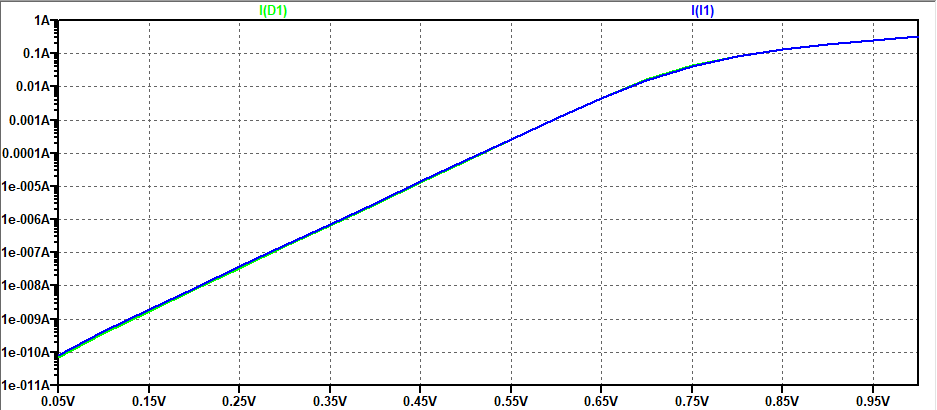
\includegraphics[width=\linewidth]{1_take_1.png}
	\caption{Подбор параметров IS и N}	
\end{figure}

\begin{figure}[H]
	\centering
	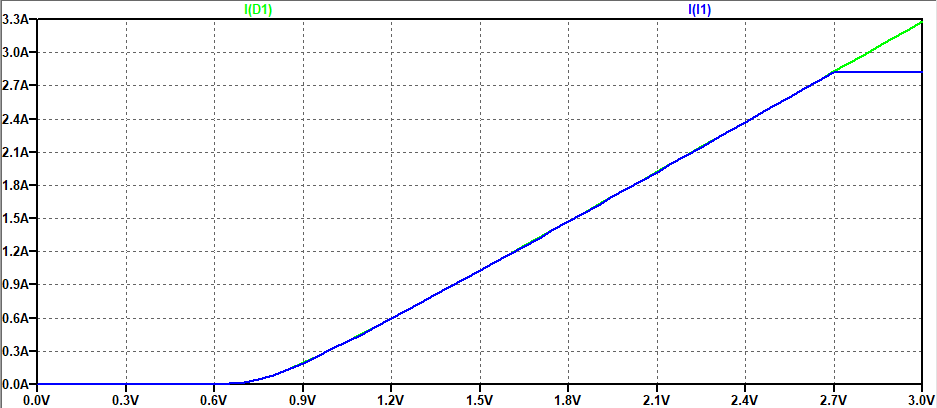
\includegraphics[width=\linewidth]{1_take_2.png}
	\caption{Подбор параметра RS}	
\end{figure}

\begin{figure}[H]
	\centering
	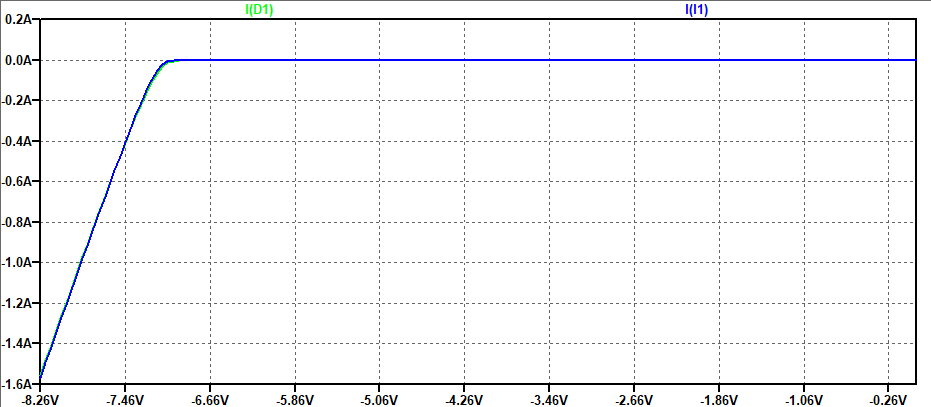
\includegraphics[width=\linewidth]{1_take_3.png}
	\caption{Подбор параметров BV NBV}	
\end{figure}

\begin{figure}[H]
	\centering
	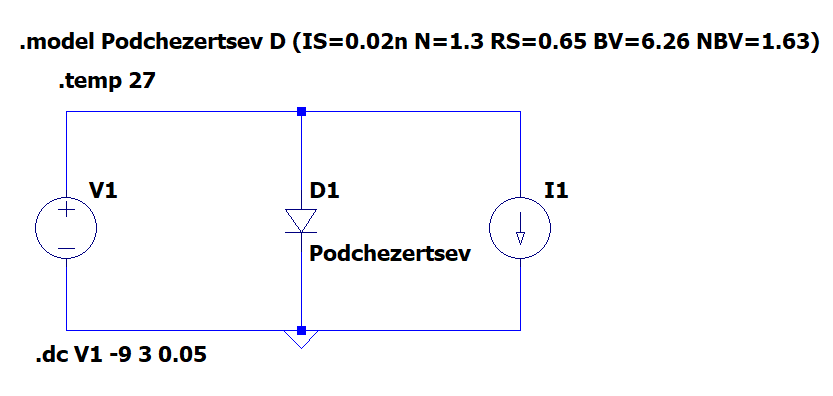
\includegraphics[width=\linewidth]{1_scema.png}
	\caption{Итоговая схема}	
\end{figure}

\section{Задание. Исследование однофазного однополупериодного выпрямителя}

\subsection{Конденсатор отсутствует}
\begin{figure}[H]
	\centering
	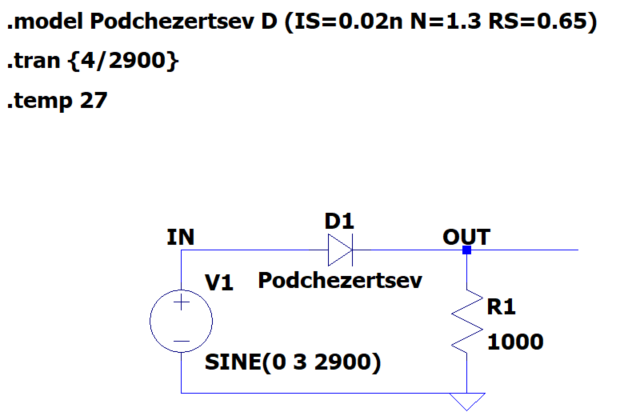
\includegraphics[width=\linewidth]{2_A_scema.png}
	\caption{Схема для задания}	
\end{figure}

\begin{figure}[H]
	\centering
	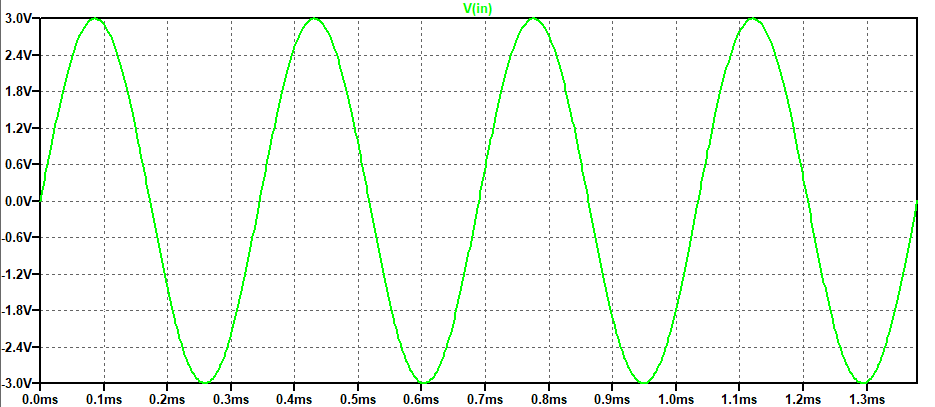
\includegraphics[width=\linewidth]{2_A_Vin.png}
	\caption{Входное напряжение}	
\end{figure}

\begin{figure}[H]
	\centering
	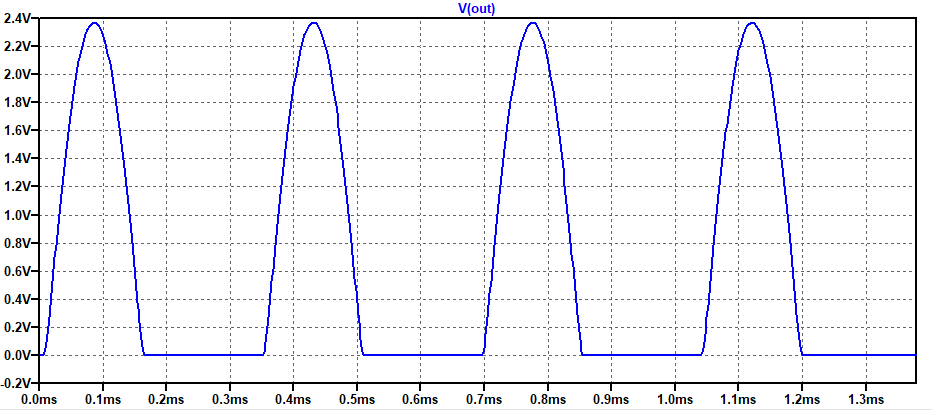
\includegraphics[width=\linewidth]{2_A_Vout.png}
	\caption{Выходное напряжение}	
\end{figure}

\begin{figure}[H]
	\centering
	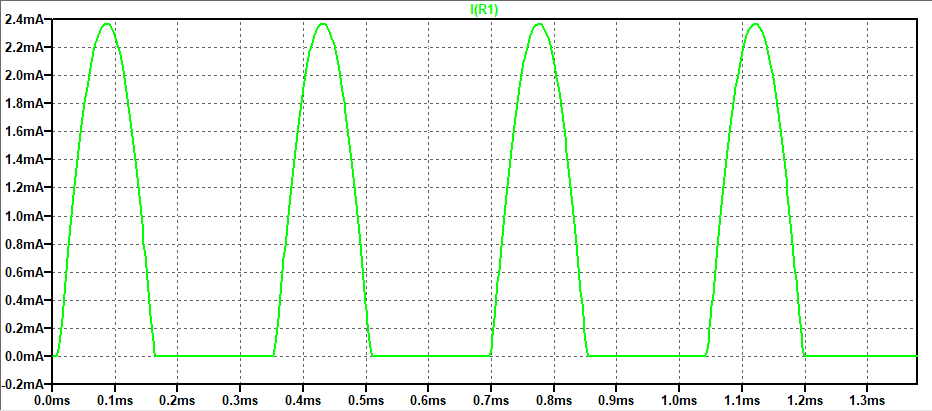
\includegraphics[width=\linewidth]{2_A_Iin.png}
	\caption{Входной ток}	
\end{figure}

\begin{figure}[H]
	\centering
	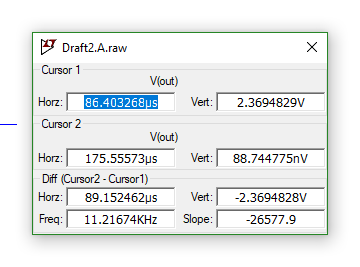
\includegraphics[]{2_A_Diff.png}
	\caption{Данные размаха напряжения}	
\end{figure}

\begin{figure}[H]
	\centering
	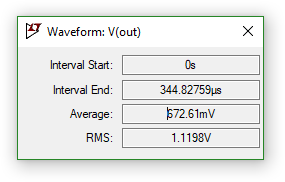
\includegraphics[]{2_A_Avr.png}
	\caption{Среднее значение напряжения}	
\end{figure}

$$k = \frac{2.3695}{0.6726} = 3.522896$$

\subsection{Конденсатор присутствует, $C = 4.7$ мкФ}
\begin{figure}[H]
	\centering
	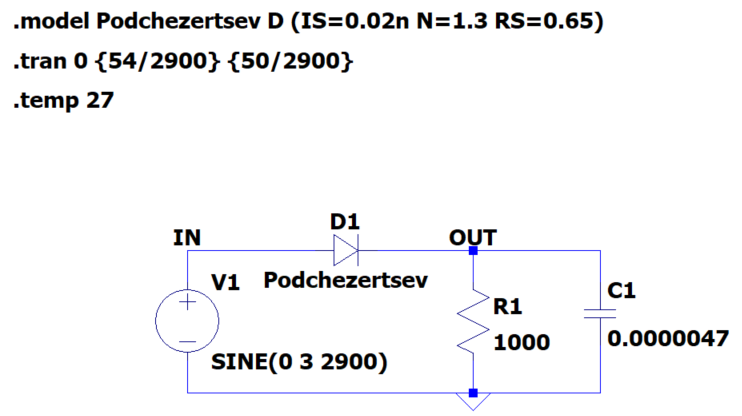
\includegraphics[width=\linewidth]{2_B_scema.png}
	\caption{Схема для задания}	
\end{figure}

\begin{figure}[H]
	\centering
	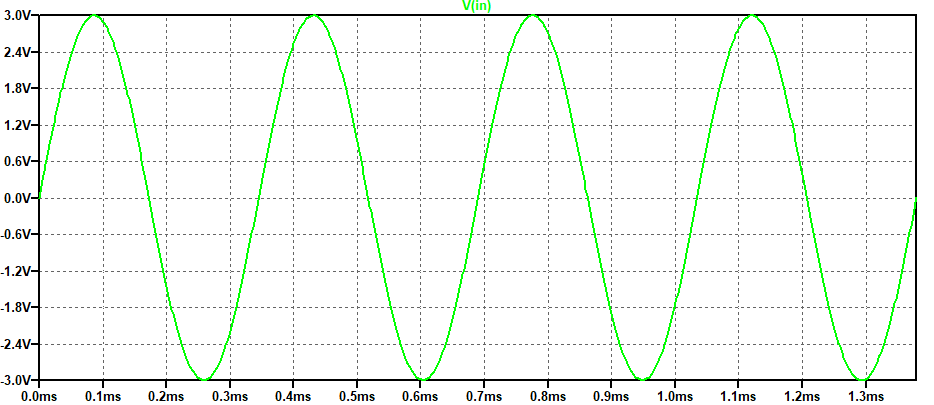
\includegraphics[width=\linewidth]{2_B_Vin.png}
	\caption{Входное напряжение}	
\end{figure}

\begin{figure}[H]
	\centering
	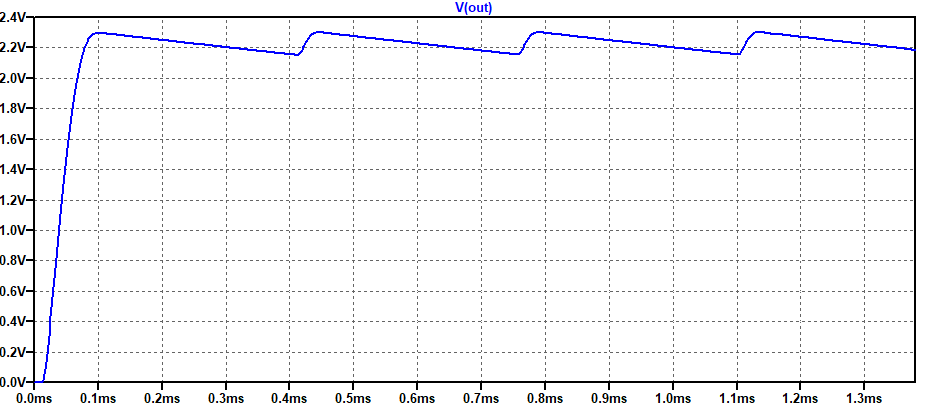
\includegraphics[width=\linewidth]{2_B_Vout.png}
	\caption{Выходное напряжение}	
\end{figure}

\begin{figure}[H]
	\centering
	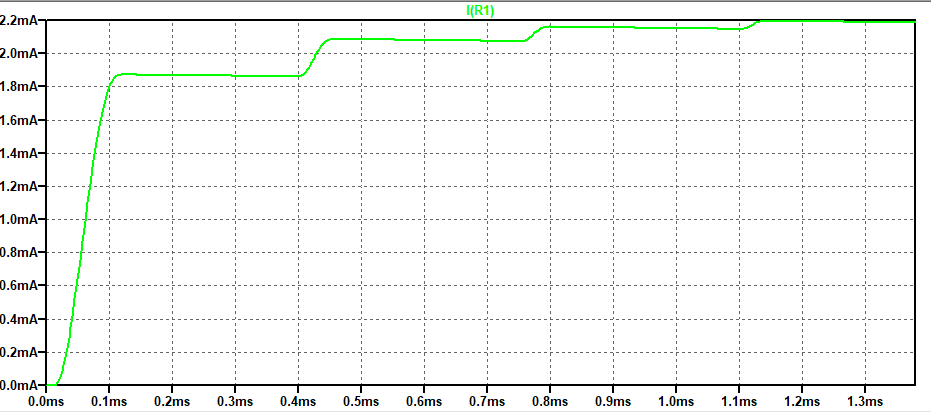
\includegraphics[width=\linewidth]{2_B_Iin.png}
	\caption{Входной ток}	
\end{figure}

\begin{figure}[H]
	\centering
	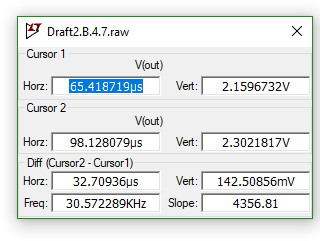
\includegraphics[]{2_B_Diff.png}
	\caption{Данные размаха напряжения}	
\end{figure}

\begin{figure}[H]
	\centering
	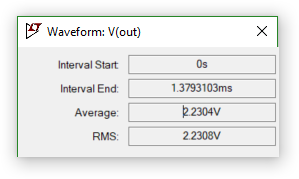
\includegraphics[]{2_B_Avr.png}
	\caption{Среднее значение напряжения}	
\end{figure}

$$k = \frac{0.1417}{2.2304} = 0.063531$$

\subsection{Конденсатор присутствует, $C = 47$ мкФ}
\begin{figure}[H]
	\centering
	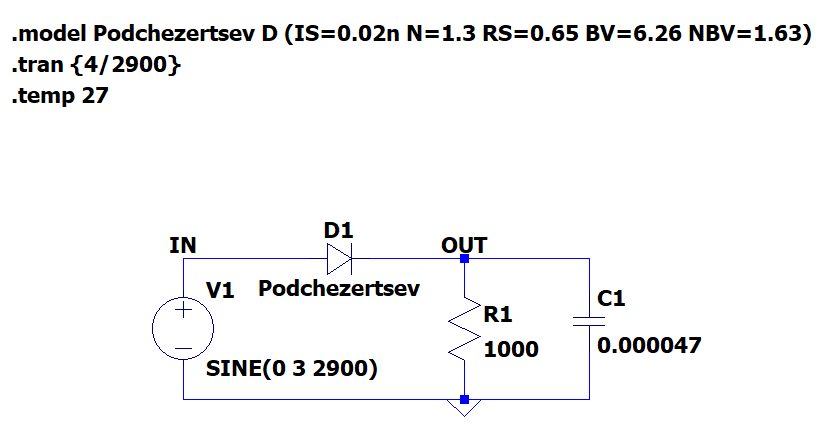
\includegraphics[width=\linewidth]{2_C_scema.png}
	\caption{Схема для задания}	
\end{figure}

\begin{figure}[H]
	\centering
	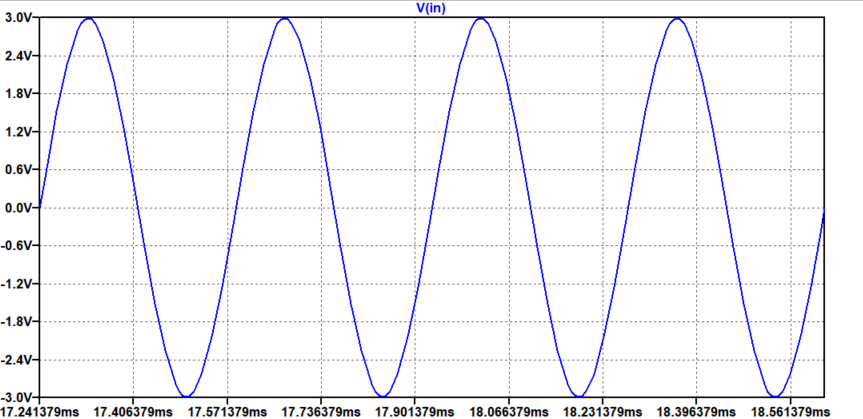
\includegraphics[width=\linewidth]{2_C_Vin.png}
	\caption{Входное напряжение}	
\end{figure}

\begin{figure}[H]
	\centering
	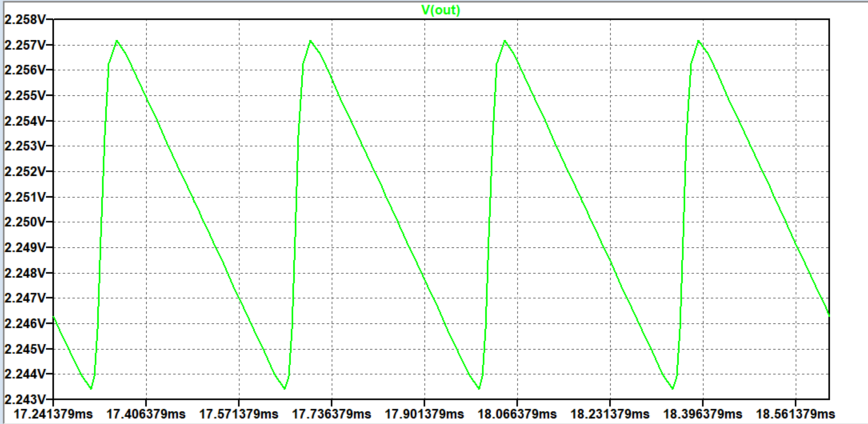
\includegraphics[width=\linewidth]{2_C_Vout.png}
	\caption{Выходное напряжение}	
\end{figure}

\begin{figure}[H]
	\centering
	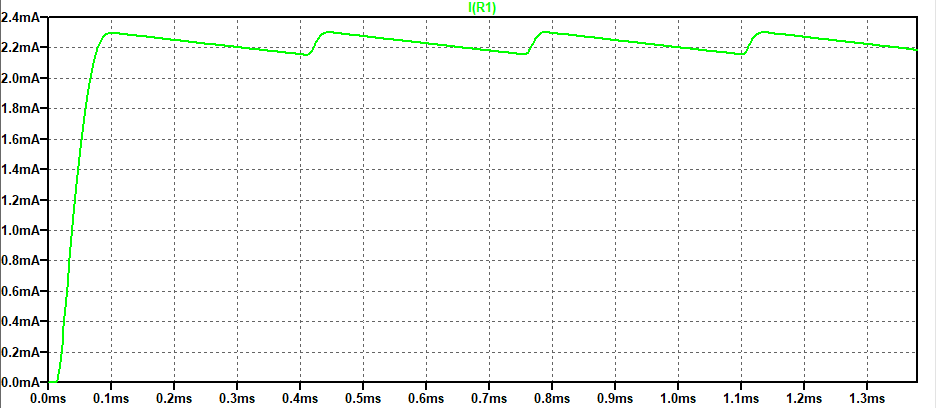
\includegraphics[width=\linewidth]{2_C_Iin.png}
	\caption{Входной ток}	
\end{figure}

\begin{figure}[H]
	\centering
	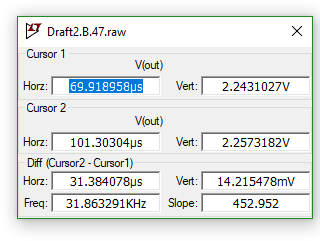
\includegraphics[]{2_C_Diff.png}
	\caption{Данные размаха напряжения}	
\end{figure}

\begin{figure}[H]
	\centering
	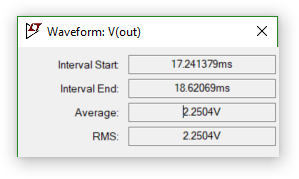
\includegraphics[]{2_C_Avr.png}
	\caption{Среднее значение напряжения}	
\end{figure}

$$k = \frac{0.01362}{2.2504} = 0.006052$$

\section{Задание. Исследование мостового выпрямителя}

\subsection{Конденсатор отсутствует}
\begin{figure}[H]
	\centering
	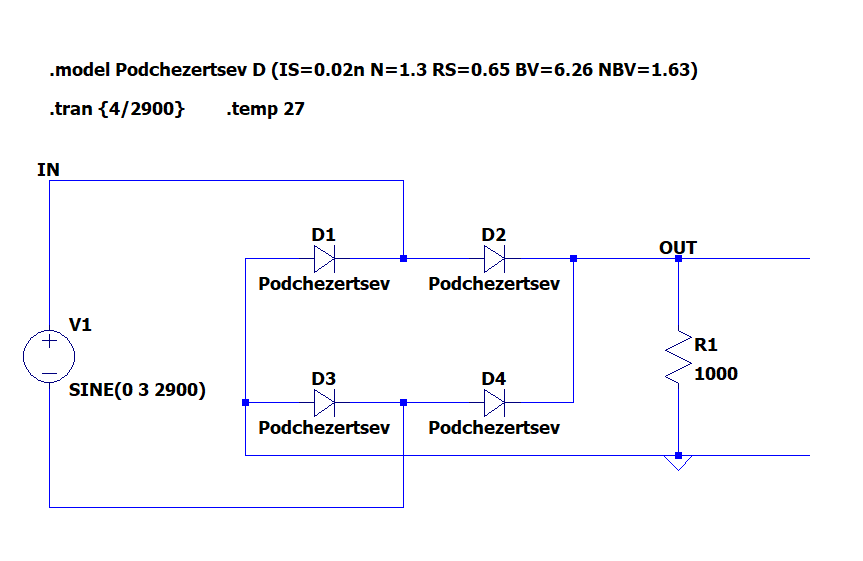
\includegraphics[width=\linewidth]{3_A_scema.png}
	\caption{Схема для задания}	
\end{figure}

\begin{figure}[H]
	\centering
	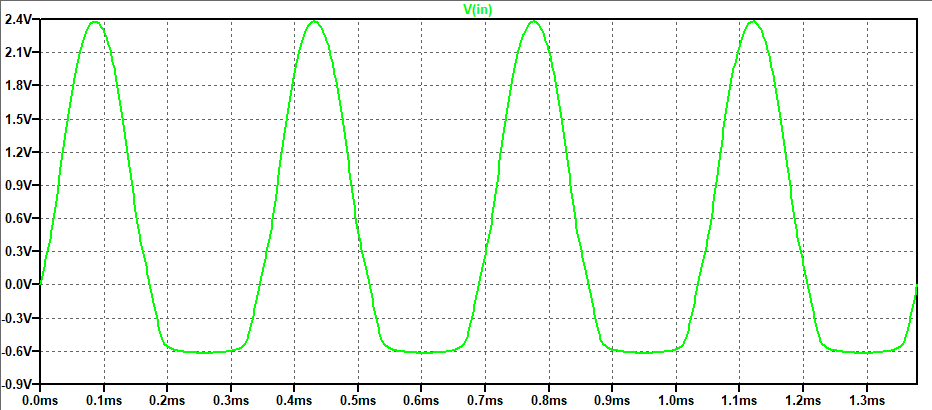
\includegraphics[width=\linewidth]{3_A_Vin.png}
	\caption{Входное напряжение}	
\end{figure}

\begin{figure}[H]
	\centering
	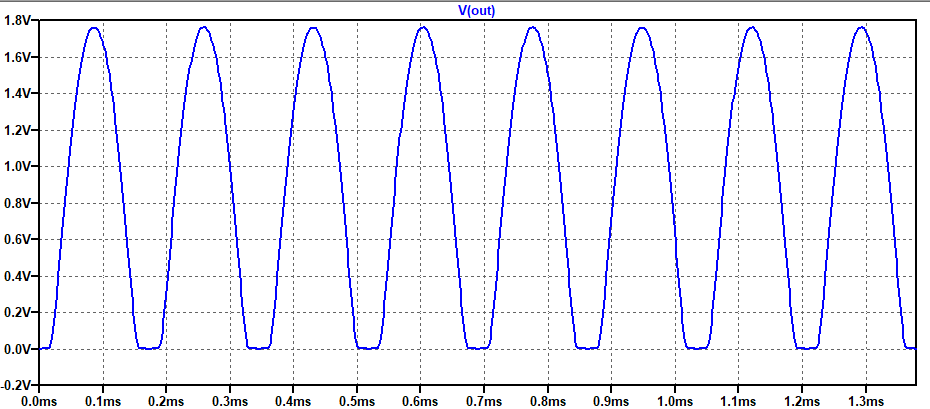
\includegraphics[width=\linewidth]{3_A_Vout.png}
	\caption{Выходное напряжение}	
\end{figure}

\begin{figure}[H]
	\centering
	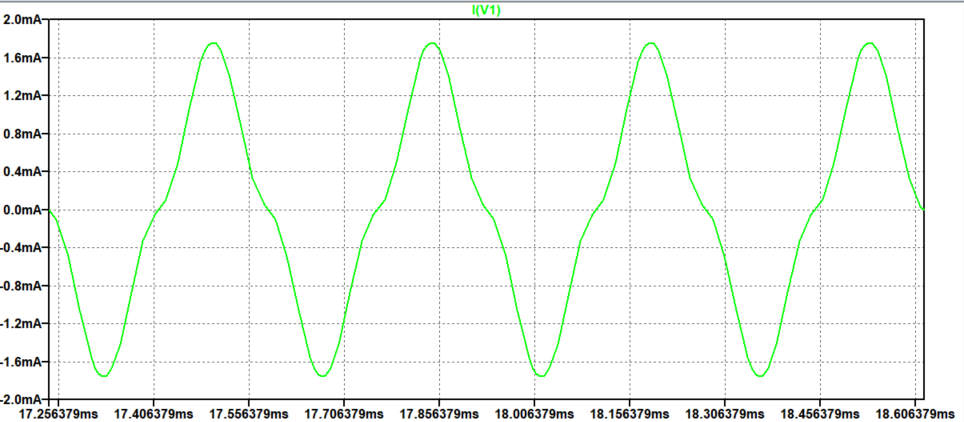
\includegraphics[width=\linewidth]{3_A_Iin.png}
	\caption{Входной ток}	
\end{figure}

\begin{figure}[H]
	\centering
	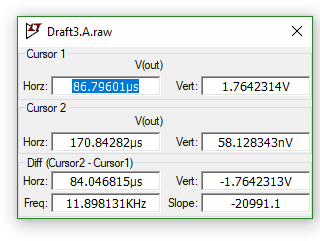
\includegraphics[]{3_A_Diff.png}
	\caption{Данные размаха напряжения}	
\end{figure}

\begin{figure}[H]
	\centering
	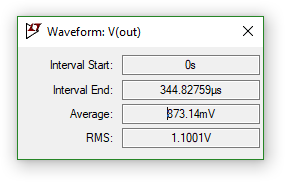
\includegraphics[]{3_A_Avr.png}
	\caption{Среднее значение напряжения}	
\end{figure}

$$k = \frac{1.69177}{0.89786} = 1.884224$$

\subsection{Конденсатор присутствует, $C = 4.7$ мкФ}
\begin{figure}[H]
	\centering
	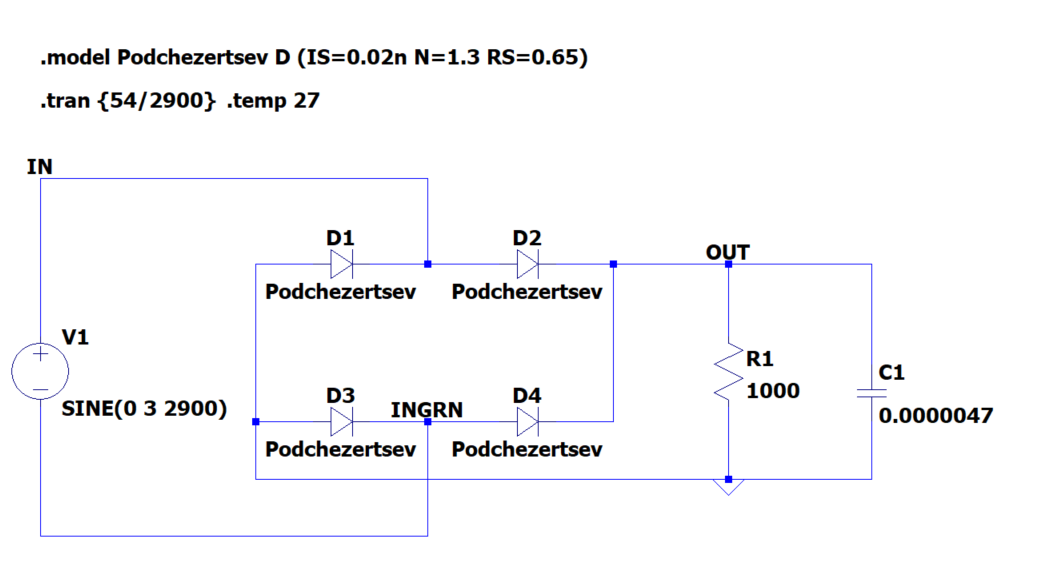
\includegraphics[width=\linewidth]{3_B_scema.png}
	\caption{Схема для задания}	
\end{figure}

\begin{figure}[H]
	\centering
	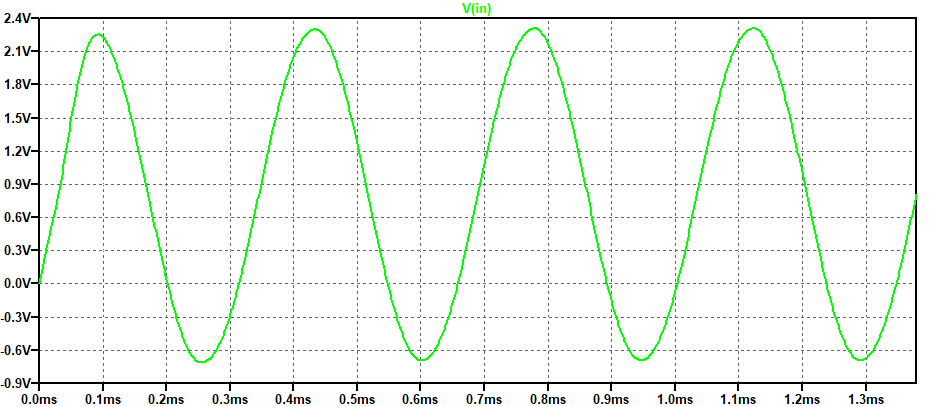
\includegraphics[width=\linewidth]{3_B_Vin.png}
	\caption{Входное напряжение}	
\end{figure}

\begin{figure}[H]
	\centering
	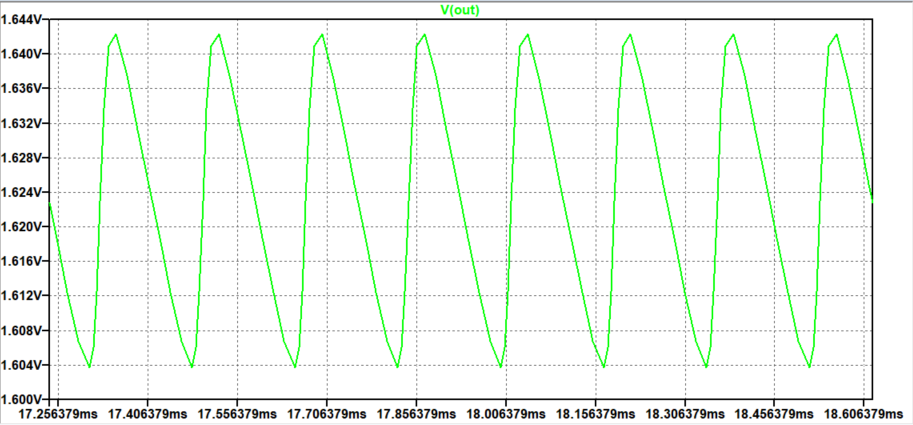
\includegraphics[width=\linewidth]{3_B_Vout.png}
	\caption{Выходное напряжение}	
\end{figure}

\begin{figure}[H]
	\centering
	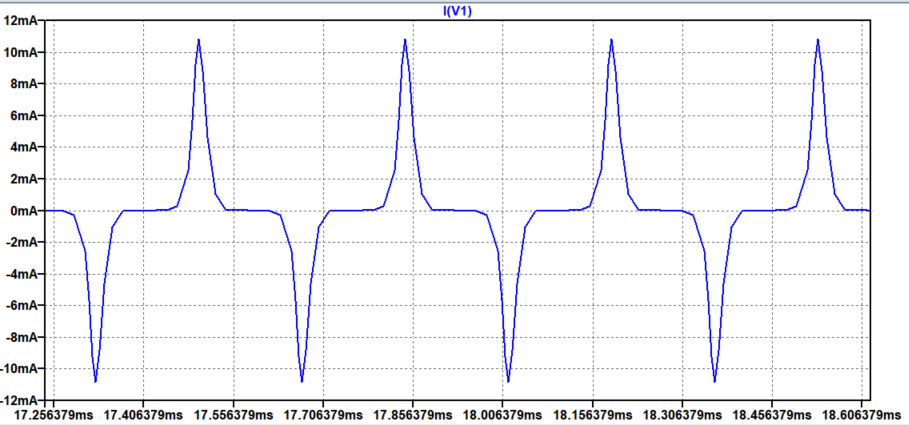
\includegraphics[width=\linewidth]{3_B_Iin.png}
	\caption{Входной ток}	
\end{figure}

\begin{figure}[H]
	\centering
	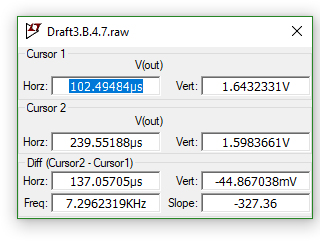
\includegraphics[]{3_B_Diff.png}
	\caption{Данные размаха напряжения}	
\end{figure}

\begin{figure}[H]
	\centering
	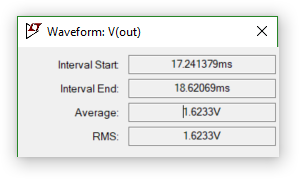
\includegraphics[]{3_B_Avr.png}
	\caption{Среднее значение напряжения}	
\end{figure}

$$k = \frac{0.03819}{1.6233} = 0.023526$$

\subsection{Конденсатор присутствует, $C = 47$ мкФ}
\begin{figure}[H]
	\centering
	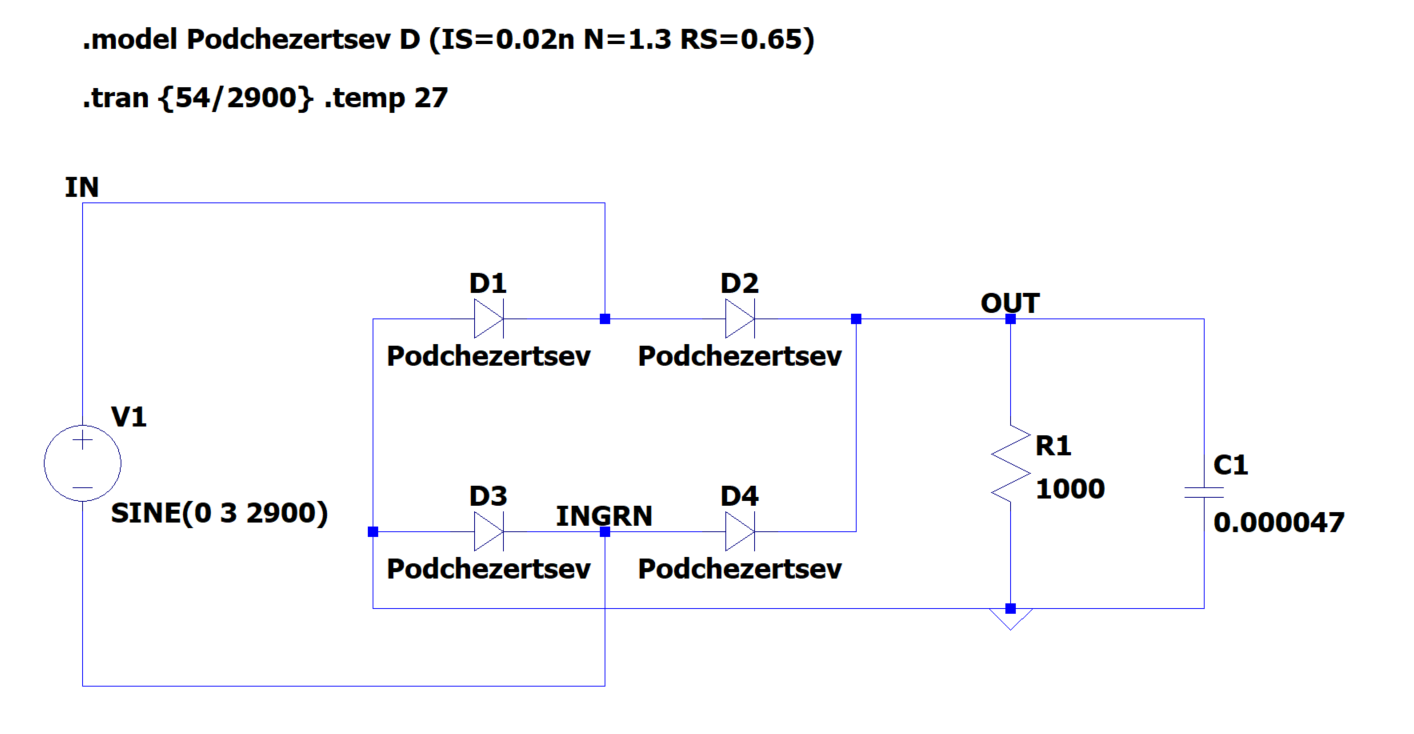
\includegraphics[width=\linewidth]{3_C_scema.png}
	\caption{Схема для задания}	
\end{figure}

\begin{figure}[H]
	\centering
	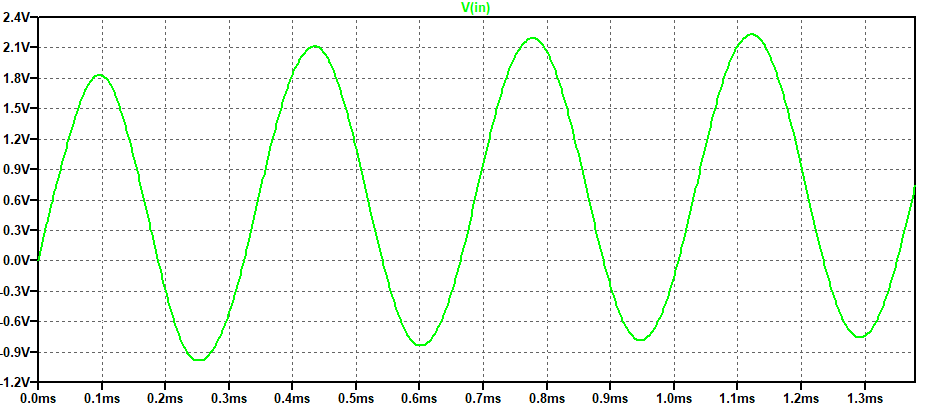
\includegraphics[width=\linewidth]{3_C_Vin.png}
	\caption{Входное напряжение}	
\end{figure}

\begin{figure}[H]
	\centering
	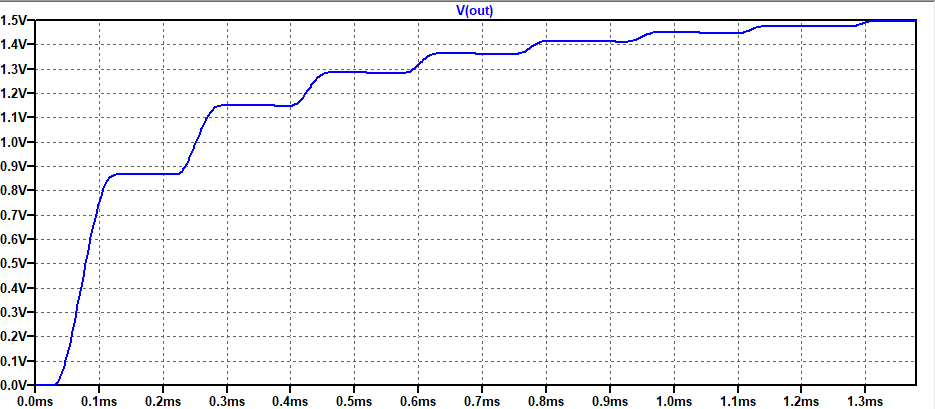
\includegraphics[width=\linewidth]{3_C_Vout.png}
	\caption{Выходное напряжение}	
\end{figure}

\begin{figure}[H]
	\centering
	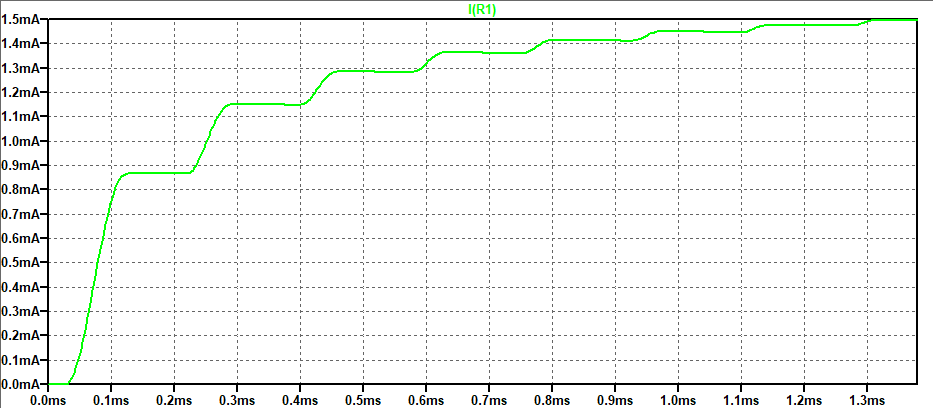
\includegraphics[width=\linewidth]{3_C_Iin.png}
	\caption{Входной ток}	
\end{figure}

\begin{figure}[H]
	\centering
	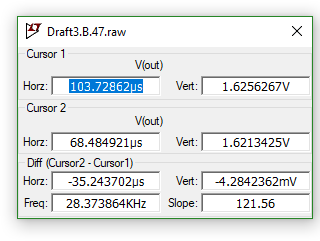
\includegraphics[]{3_C_Diff.png}
	\caption{Данные размаха напряжения}	
\end{figure}

\begin{figure}[H]
	\centering
	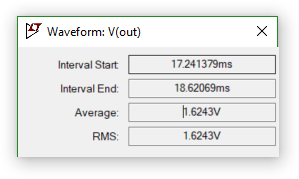
\includegraphics[]{3_C_Avr.png}
	\caption{Среднее значение напряжения}	
\end{figure}

$$k = \frac{0.003898}{1.6243} = 0.0023998$$

\section{Анализ результатов}

\begin{table}[H]
	\begin{center}
	\tablecaption{Результаты вычислений коэффициента пульсации в различных случаях}
	\begin{tabular}{|c|c|c|}
		\hline
		\multirow{2}{*}{Емкость, мкФ} & \multicolumn{2}{c|}{Выпрямитель} \\ \cline{2-3} 
		& Однополупериодный   & Мостовой   \\ \hline
		Отсутствует              & 3.522896            & 1.884224   \\ \hline
		4.7                      & 0.063531            & 0.023526   \\ \hline
		47                       & 0.006052            & 0.002400   \\ \hline
	\end{tabular}
	\end{center}
\end{table}

\begin{itemize}
	\item Мостовой выпрямитель по характеристикам лучше однофазного однополупериодного выпрямителя;
	\item Наличие нагрузочной ёмкости значительно уменьшает коэффициент пульсации;
	\item Чем больше емкость -- тем меньше коэффициент пульсации.
\end{itemize}

\section{Исходные данные}

\begin{longtable}{|l|l|}

\caption{}\\
\hline
Voltage, V & Current, A \\ \hline
\endfirsthead
\hline
Voltage, V & Current, A \\ \hline
\endhead
\hline
\multicolumn{2}{r}{продолжение следует\ldots} \
\endfoot
\hline
\endlastfoot		
-12.0000000000000000	&	-7.2422000000000000\\ \hline
-11.9500000000000000	&	-7.1658000000000000\\ \hline
-11.9000000000000000	&	-7.0895000000000000\\ \hline
-11.8500000000000000	&	-7.0131000000000000\\ \hline
-11.8000000000000000	&	-6.9367000000000000\\ \hline
-11.7500000000000000	&	-6.8604000000000000\\ \hline
-11.7000000000000000	&	-6.7841000000000000\\ \hline
-11.6500000000000000	&	-6.7077000000000000\\ \hline
-11.6000000000000000	&	-6.6314000000000000\\ \hline
-11.5500000000000000	&	-6.5551000000000000\\ \hline
-11.5000000000000000	&	-6.4788000000000000\\ \hline
-11.4500000000000000	&	-6.4025000000000000\\ \hline
-11.4000000000000000	&	-6.3262000000000000\\ \hline
-11.3500000000000000	&	-6.2499000000000000\\ \hline
-11.3000000000000000	&	-6.1736000000000000\\ \hline
-11.2500000000000000	&	-6.0973000000000000\\ \hline
-11.2000000000000000	&	-6.0211000000000000\\ \hline
-11.1500000000000000	&	-5.9448000000000000\\ \hline
-11.1000000000000000	&	-5.8685000000000000\\ \hline
-11.0500000000000000	&	-5.7923000000000000\\ \hline
-11.0000000000000000	&	-5.7161000000000000\\ \hline
-10.9500000000000000	&	-5.6399000000000000\\ \hline
-10.9000000000000000	&	-5.5636000000000000\\ \hline
-10.8500000000000000	&	-5.4874000000000000\\ \hline
-10.8000000000000000	&	-5.4112000000000000\\ \hline
-10.7500000000000000	&	-5.3351000000000000\\ \hline
-10.7000000000000000	&	-5.2589000000000000\\ \hline
-10.6500000000000000	&	-5.1827000000000000\\ \hline
-10.6000000000000000	&	-5.1066000000000000\\ \hline
-10.5500000000000000	&	-5.0304000000000000\\ \hline
-10.5000000000000000	&	-4.9543000000000000\\ \hline
-10.4500000000000000	&	-4.8782000000000000\\ \hline
-10.4000000000000000	&	-4.8021000000000000\\ \hline
-10.3500000000000000	&	-4.7260000000000000\\ \hline
-10.3000000000000000	&	-4.6499000000000000\\ \hline
-10.2500000000000000	&	-4.5739000000000000\\ \hline
-10.2000000000000000	&	-4.4978000000000000\\ \hline
-10.1500000000000000	&	-4.4218000000000000\\ \hline
-10.1000000000000000	&	-4.3458000000000000\\ \hline
-10.0500000000000000	&	-4.2698000000000000\\ \hline
-10.0000000000000000	&	-4.1938000000000000\\ \hline
-9.9500000000000000	&	-4.1178000000000000\\ \hline
-9.9000000000000000	&	-4.0419000000000000\\ \hline
-9.8500000000000000	&	-3.9659000000000000\\ \hline
-9.8000000000000000	&	-3.8900000000000000\\ \hline
-9.7500000000000000	&	-3.8141000000000000\\ \hline
-9.7000000000000000	&	-3.7382000000000000\\ \hline
-9.6500000000000000	&	-3.6624000000000000\\ \hline
-9.6000000000000000	&	-3.5866000000000000\\ \hline
-9.5500000000000000	&	-3.5108000000000000\\ \hline
-9.5000000000000000	&	-3.4350000000000000\\ \hline
-9.4500000000000000	&	-3.3592000000000000\\ \hline
-9.4000000000000000	&	-3.2835000000000000\\ \hline
-9.3500000000000000	&	-3.2078000000000000\\ \hline
-9.3000000000000000	&	-3.1321000000000000\\ \hline
-9.2500000000000000	&	-3.0564000000000000\\ \hline
-9.2000000000000000	&	-2.9808000000000000\\ \hline
-9.1500000000000000	&	-2.9053000000000000\\ \hline
-9.1000000000000000	&	-2.8297000000000000\\ \hline
-9.0500000000000000	&	-2.7542000000000000\\ \hline
-9.0000000000000000	&	-2.6787000000000000\\ \hline
-8.9500000000000000	&	-2.6033000000000000\\ \hline
-8.9000000000000000	&	-2.5279000000000000\\ \hline
-8.8500000000000000	&	-2.4526000000000000\\ \hline
-8.8000000000000000	&	-2.3773000000000000\\ \hline
-8.7500000000000000	&	-2.3020000000000000\\ \hline
-8.7000000000000000	&	-2.2268000000000000\\ \hline
-8.6500000000000000	&	-2.1517000000000000\\ \hline
-8.6000000000000000	&	-2.0766000000000000\\ \hline
-8.5500000000000000	&	-2.0016000000000000\\ \hline
-8.5000000000000000	&	-1.9267000000000000\\ \hline
-8.4500000000000000	&	-1.8518000000000000\\ \hline
-8.4000000000000000	&	-1.7771000000000000\\ \hline
-8.3500000000000000	&	-1.7024000000000000\\ \hline
-8.3000000000000000	&	-1.6278000000000000\\ \hline
-8.2500000000000000	&	-1.5533000000000000\\ \hline
-8.2000000000000000	&	-1.4790000000000000\\ \hline
-8.1500000000000000	&	-1.4047000000000000\\ \hline
-8.1000000000000000	&	-1.3306000000000000\\ \hline
-8.0500000000000000	&	-1.2567000000000000\\ \hline
-8.0000000000000000	&	-1.1829000000000000\\ \hline
-7.9500000000000000	&	-1.1094000000000000\\ \hline
-7.9000000000000000	&	-1.0360000000000000\\ \hline
-7.8500000000000000	&	-0.9629018000000000\\ \hline
-7.8000000000000000	&	-0.8900838000000000\\ \hline
-7.7500000000000000	&	-0.8175952000000000\\ \hline
-7.7000000000000000	&	-0.7454917000000000\\ \hline
-7.6500000000000000	&	-0.6738434000000000\\ \hline
-7.6000000000000000	&	-0.6027413000000000\\ \hline
-7.5500000000000000	&	-0.5323052000000000\\ \hline
-7.5000000000000000	&	-0.4626975000000000\\ \hline
-7.4500000000000000	&	-0.3941471000000000\\ \hline
-7.4000000000000000	&	-0.3269774000000000\\ \hline
-7.3500000000000000	&	-0.2616830000000000\\ \hline
-7.3000000000000000	&	-0.1990434000000000\\ \hline
-7.2500000000000000	&	-0.1403569000000000\\ \hline
-7.2000000000000000	&	-0.0878777000000000\\ \hline
-7.1500000000000000	&	-0.0454147000000000\\ \hline
-7.1000000000000000	&	-0.0176954000000000\\ \hline
-7.0500000000000000	&	-0.0051552000000000\\ \hline
-7.0000000000000000	&	-0.0012723000000000\\ \hline
-6.9500000000000000	&	-0.0002970142000000\\ \hline
-6.9000000000000000	&	-0.0000683499000000\\ \hline
-6.8500000000000000	&	-0.0000156760000000\\ \hline
-6.8000000000000000	&	-0.0000035925000000\\ \hline
-6.7500000000000000	&	-0.0000008231506000\\ \hline
-6.7000000000000000	&	-0.0000001886058000\\ \hline
-6.6500000000000000	&	-0.0000000432182000\\ \hline
-6.6000000000000000	&	-0.0000000099071000\\ \hline
-6.5500000000000000	&	-0.0000000022749000\\ \hline
-6.5000000000000000	&	-0.0000000005262280\\ \hline
-6.4500000000000000	&	-0.0000000001255280\\ \hline
-6.4000000000000000	&	-0.0000000000336833\\ \hline
-6.3500000000000000	&	-0.0000000000302656\\ \hline
-6.3000000000000000	&	-0.0000000000302158\\ \hline
-6.2500000000000000	&	-0.0000000000301661\\ \hline
-6.2000000000000000	&	-0.0000000000301146\\ \hline
-6.1500000000000000	&	-0.0000000000300648\\ \hline
-6.1000000000000000	&	-0.0000000000300151\\ \hline
-6.0500000000000000	&	-0.0000000000299654\\ \hline
-6.0000000000000000	&	-0.0000000000299156\\ \hline
-5.9500000000000000	&	-0.0000000000298659\\ \hline
-5.9000000000000000	&	-0.0000000000298161\\ \hline
-5.8500000000000000	&	-0.0000000000297646\\ \hline
-5.8000000000000000	&	-0.0000000000297149\\ \hline
-5.7500000000000000	&	-0.0000000000296652\\ \hline
-5.7000000000000000	&	-0.0000000000296154\\ \hline
-5.6500000000000000	&	-0.0000000000295657\\ \hline
-5.6000000000000000	&	-0.0000000000295159\\ \hline
-5.5500000000000000	&	-0.0000000000294662\\ \hline
-5.5000000000000000	&	-0.0000000000294147\\ \hline
-5.4500000000000000	&	-0.0000000000293650\\ \hline
-5.4000000000000000	&	-0.0000000000293152\\ \hline
-5.3500000000000000	&	-0.0000000000292655\\ \hline
-5.3000000000000000	&	-0.0000000000292157\\ \hline
-5.2500000000000000	&	-0.0000000000291660\\ \hline
-5.2000000000000000	&	-0.0000000000291154\\ \hline
-5.1500000000000000	&	-0.0000000000290656\\ \hline
-5.1000000000000000	&	-0.0000000000290150\\ \hline
-5.0500000000000000	&	-0.0000000000289653\\ \hline
-5.0000000000000000	&	-0.0000000000289155\\ \hline
-4.9500000000000000	&	-0.0000000000288658\\ \hline
-4.9000000000000000	&	-0.0000000000288152\\ \hline
-4.8500000000000000	&	-0.0000000000287654\\ \hline
-4.8000000000000000	&	-0.0000000000287157\\ \hline
-4.7500000000000000	&	-0.0000000000286651\\ \hline
-4.7000000000000000	&	-0.0000000000286153\\ \hline
-4.6500000000000000	&	-0.0000000000285656\\ \hline
-4.6000000000000000	&	-0.0000000000285150\\ \hline
-4.5500000000000000	&	-0.0000000000284652\\ \hline
-4.5000000000000000	&	-0.0000000000284155\\ \hline
-4.4500000000000000	&	-0.0000000000283658\\ \hline
-4.4000000000000000	&	-0.0000000000283151\\ \hline
-4.3500000000000000	&	-0.0000000000282654\\ \hline
-4.3000000000000000	&	-0.0000000000282157\\ \hline
-4.2500000000000000	&	-0.0000000000281650\\ \hline
-4.2000000000000000	&	-0.0000000000281153\\ \hline
-4.1500000000000000	&	-0.0000000000280655\\ \hline
-4.1000000000000000	&	-0.0000000000280149\\ \hline
-4.0500000000000000	&	-0.0000000000279652\\ \hline
-4.0000000000000000	&	-0.0000000000279154\\ \hline
-3.9500000000000000	&	-0.0000000000278657\\ \hline
-3.9000000000000000	&	-0.0000000000278151\\ \hline
-3.8500000000000000	&	-0.0000000000277653\\ \hline
-3.8000000000000000	&	-0.0000000000277156\\ \hline
-3.7500000000000000	&	-0.0000000000276650\\ \hline
-3.7000000000000000	&	-0.0000000000276152\\ \hline
-3.6500000000000000	&	-0.0000000000275655\\ \hline
-3.6000000000000000	&	-0.0000000000275149\\ \hline
-3.5500000000000000	&	-0.0000000000274651\\ \hline
-3.5000000000000000	&	-0.0000000000274154\\ \hline
-3.4500000000000000	&	-0.0000000000273657\\ \hline
-3.4000000000000000	&	-0.0000000000273150\\ \hline
-3.3500000000000000	&	-0.0000000000272653\\ \hline
-3.3000000000000000	&	-0.0000000000272156\\ \hline
-3.2500000000000000	&	-0.0000000000271649\\ \hline
-3.2000000000000000	&	-0.0000000000271152\\ \hline
-3.1500000000000000	&	-0.0000000000270655\\ \hline
-3.1000000000000000	&	-0.0000000000270148\\ \hline
-3.0500000000000000	&	-0.0000000000269651\\ \hline
-3.0000000000000000	&	-0.0000000000269154\\ \hline
-2.9500000000000000	&	-0.0000000000268656\\ \hline
-2.9000000000000000	&	-0.0000000000268150\\ \hline
-2.8500000000000000	&	-0.0000000000267653\\ \hline
-2.8000000000000000	&	-0.0000000000267155\\ \hline
-2.7500000000000000	&	-0.0000000000266649\\ \hline
-2.7000000000000000	&	-0.0000000000266152\\ \hline
-2.6500000000000000	&	-0.0000000000265654\\ \hline
-2.6000000000000000	&	-0.0000000000265157\\ \hline
-2.5500000000000000	&	-0.0000000000264655\\ \hline
-2.5000000000000000	&	-0.0000000000264158\\ \hline
-2.4500000000000000	&	-0.0000000000263656\\ \hline
-2.4000000000000000	&	-0.0000000000263158\\ \hline
-2.3500000000000000	&	-0.0000000000262657\\ \hline
-2.3000000000000000	&	-0.0000000000262155\\ \hline
-2.2500000000000000	&	-0.0000000000261657\\ \hline
-2.2000000000000000	&	-0.0000000000261156\\ \hline
-2.1500000000000000	&	-0.0000000000260658\\ \hline
-2.1000000000000000	&	-0.0000000000260156\\ \hline
-2.0500000000000000	&	-0.0000000000259655\\ \hline
-2.0000000000000000	&	-0.0000000000259157\\ \hline
-1.9500000000000000	&	-0.0000000000258655\\ \hline
-1.9000000000000000	&	-0.0000000000258158\\ \hline
-1.8500000000000000	&	-0.0000000000257656\\ \hline
-1.8000000000000000	&	-0.0000000000257154\\ \hline
-1.7500000000000000	&	-0.0000000000256657\\ \hline
-1.7000000000000000	&	-0.0000000000256155\\ \hline
-1.6500000000000000	&	-0.0000000000255658\\ \hline
-1.6000000000000000	&	-0.0000000000255156\\ \hline
-1.5500000000000000	&	-0.0000000000254654\\ \hline
-1.5000000000000000	&	-0.0000000000254157\\ \hline
-1.4500000000000000	&	-0.0000000000253655\\ \hline
-1.4000000000000000	&	-0.0000000000253157\\ \hline
-1.3500000000000000	&	-0.0000000000252656\\ \hline
-1.3000000000000000	&	-0.0000000000252154\\ \hline
-1.2500000000000000	&	-0.0000000000251654\\ \hline
-1.2000000000000000	&	-0.0000000000251155\\ \hline
-1.1500000000000000	&	-0.0000000000250653\\ \hline
-1.1000000000000000	&	-0.0000000000250153\\ \hline
-1.0500000000000000	&	-0.0000000000249654\\ \hline
-1.0000000000000000	&	-0.0000000000249154\\ \hline
-0.9500000000000000	&	-0.0000000000248654\\ \hline
-0.9000000000000000	&	-0.0000000000248153\\ \hline
-0.8500000000000000	&	-0.0000000000247653\\ \hline
-0.8000000000000000	&	-0.0000000000247153\\ \hline
-0.7500000000000000	&	-0.0000000000246654\\ \hline
-0.7000000000000000	&	-0.0000000000246154\\ \hline
-0.6500000000000000	&	-0.0000000000245653\\ \hline
-0.6000000000000000	&	-0.0000000000245154\\ \hline
-0.5500000000000000	&	-0.0000000000244653\\ \hline
-0.5000000000000000	&	-0.0000000000244154\\ \hline
-0.4500000000000000	&	-0.0000000000243653\\ \hline
-0.4000000000000000	&	-0.0000000000243153\\ \hline
-0.3500000000000000	&	-0.0000000000242654\\ \hline
-0.3000000000000000	&	-0.0000000000242120\\ \hline
-0.2500000000000000	&	-0.0000000000241503\\ \hline
-0.2000000000000000	&	-0.0000000000240495\\ \hline
-0.1500000000000000	&	-0.0000000000237777\\ \hline
-0.1000000000000000	&	-0.0000000000227599\\ \hline
-0.0500000000000000	&	-0.0000000000184859\\ \hline
0.0000000000000000	&	0.0000000000000000\\ \hline
0.0500000000000000	&	0.0000000000805149\\ \hline
0.1000000000000000	&	0.0000000004317595\\ \hline
0.1500000000000000	&	0.0000000019646000\\ \hline
0.2000000000000000	&	0.0000000086547000\\ \hline
0.2500000000000000	&	0.0000000378540000\\ \hline
0.3000000000000000	&	0.0000001652958000\\ \hline
0.3500000000000000	&	0.0000007215168000\\ \hline
0.4000000000000000	&	0.0000031490000000\\ \hline
0.4500000000000000	&	0.0000137415000000\\ \hline
0.5000000000000000	&	0.0000599228000000\\ \hline
0.5500000000000000	&	0.0002605341000000\\ \hline
0.6000000000000000	&	0.0011186000000000\\ \hline
0.6500000000000000	&	0.0045698000000000\\ \hline
0.7000000000000000	&	0.0160177000000000\\ \hline
0.7500000000000000	&	0.0422760000000000\\ \hline
0.8000000000000000	&	0.0836028000000000\\ \hline
0.8500000000000000	&	0.1353684000000000\\ \hline
0.9000000000000000	&	0.1936106000000000\\ \hline
0.9500000000000000	&	0.2559599000000000\\ \hline
1.0000000000000000	&	0.3210542000000000\\ \hline
1.0500000000000000	&	0.3880794000000000\\ \hline
1.1000000000000000	&	0.4565231000000000\\ \hline
1.1500000000000000	&	0.5260463000000000\\ \hline
1.2000000000000000	&	0.5964140000000000\\ \hline
1.2500000000000000	&	0.6674622000000000\\ \hline
1.3000000000000000	&	0.7390658000000000\\ \hline
1.3500000000000000	&	0.8111319000000000\\ \hline
1.4000000000000000	&	0.8835885000000000\\ \hline
1.4500000000000000	&	0.9563790000000000\\ \hline
1.5000000000000000	&	1.0295000000000000\\ \hline
1.5500000000000000	&	1.1028000000000000\\ \hline
1.6000000000000000	&	1.1763000000000000\\ \hline
1.6500000000000000	&	1.2501000000000000\\ \hline
1.7000000000000000	&	1.3240000000000000\\ \hline
1.7500000000000000	&	1.3981000000000000\\ \hline
1.8000000000000000	&	1.4723000000000000\\ \hline
1.8500000000000000	&	1.5467000000000000\\ \hline
1.9000000000000000	&	1.6211000000000000\\ \hline
1.9500000000000000	&	1.6957000000000000\\ \hline
2.0000000000000000	&	1.7704000000000000\\ \hline
2.0500000000000000	&	1.8451000000000000\\ \hline
2.1000000000000000	&	1.9200000000000000\\ \hline
2.1500000000000000	&	1.9949000000000000\\ \hline
2.2000000000000000	&	2.0699000000000000\\ \hline
2.2500000000000000	&	2.1450000000000000\\ \hline
2.3000000000000000	&	2.2201000000000000\\ \hline
2.3500000000000000	&	2.2953000000000000\\ \hline
2.4000000000000000	&	2.3705000000000000\\ \hline
2.4500000000000000	&	2.4458000000000000\\ \hline
2.5000000000000000	&	2.5212000000000000\\ \hline
2.5500000000000000	&	2.5965000000000000\\ \hline
2.6000000000000000	&	2.6720000000000000\\ \hline
2.6500000000000000	&	2.7474000000000000\\ \hline
2.7000000000000000	&	2.8230000000000000\\ \hline

\end{longtable}


\end{document} % конец документа